% Options for packages loaded elsewhere
\PassOptionsToPackage{unicode}{hyperref}
\PassOptionsToPackage{hyphens}{url}
\PassOptionsToPackage{dvipsnames,svgnames*,x11names*}{xcolor}
%
\documentclass[
  12pt,
]{article}
\usepackage{amsmath,amssymb}
\usepackage{lmodern}
\usepackage{setspace}
\usepackage{ifxetex,ifluatex}
\ifnum 0\ifxetex 1\fi\ifluatex 1\fi=0 % if pdftex
  \usepackage[T1]{fontenc}
  \usepackage[utf8]{inputenc}
  \usepackage{textcomp} % provide euro and other symbols
\else % if luatex or xetex
  \usepackage{unicode-math}
  \defaultfontfeatures{Scale=MatchLowercase}
  \defaultfontfeatures[\rmfamily]{Ligatures=TeX,Scale=1}
\fi
% Use upquote if available, for straight quotes in verbatim environments
\IfFileExists{upquote.sty}{\usepackage{upquote}}{}
\IfFileExists{microtype.sty}{% use microtype if available
  \usepackage[]{microtype}
  \UseMicrotypeSet[protrusion]{basicmath} % disable protrusion for tt fonts
}{}
\makeatletter
\@ifundefined{KOMAClassName}{% if non-KOMA class
  \IfFileExists{parskip.sty}{%
    \usepackage{parskip}
  }{% else
    \setlength{\parindent}{0pt}
    \setlength{\parskip}{6pt plus 2pt minus 1pt}}
}{% if KOMA class
  \KOMAoptions{parskip=half}}
\makeatother
\usepackage{xcolor}
\IfFileExists{xurl.sty}{\usepackage{xurl}}{} % add URL line breaks if available
\IfFileExists{bookmark.sty}{\usepackage{bookmark}}{\usepackage{hyperref}}
\hypersetup{
  pdfauthor={Dmytro Perepolkin1,; Ullrika Sahlin1; Benjamin Goodrich2},
  colorlinks=true,
  linkcolor=Maroon,
  filecolor=Maroon,
  citecolor=Blue,
  urlcolor=Blue,
  pdfcreator={LaTeX via pandoc}}
\urlstyle{same} % disable monospaced font for URLs
\usepackage[margin=1in]{geometry}
\usepackage{longtable,booktabs,array}
\usepackage{calc} % for calculating minipage widths
% Correct order of tables after \paragraph or \subparagraph
\usepackage{etoolbox}
\makeatletter
\patchcmd\longtable{\par}{\if@noskipsec\mbox{}\fi\par}{}{}
\makeatother
% Allow footnotes in longtable head/foot
\IfFileExists{footnotehyper.sty}{\usepackage{footnotehyper}}{\usepackage{footnote}}
\makesavenoteenv{longtable}
\usepackage{graphicx}
\makeatletter
\def\maxwidth{\ifdim\Gin@nat@width>\linewidth\linewidth\else\Gin@nat@width\fi}
\def\maxheight{\ifdim\Gin@nat@height>\textheight\textheight\else\Gin@nat@height\fi}
\makeatother
% Scale images if necessary, so that they will not overflow the page
% margins by default, and it is still possible to overwrite the defaults
% using explicit options in \includegraphics[width, height, ...]{}
\setkeys{Gin}{width=\maxwidth,height=\maxheight,keepaspectratio}
% Set default figure placement to htbp
\makeatletter
\def\fps@figure{htbp}
\makeatother
\setlength{\emergencystretch}{3em} % prevent overfull lines
\providecommand{\tightlist}{%
  \setlength{\itemsep}{0pt}\setlength{\parskip}{0pt}}
\setcounter{secnumdepth}{5}
\usepackage{dcolumn}
\usepackage{longtable}
\usepackage{natbib}
\usepackage{geometry}
\usepackage{lscape}
\usepackage{booktabs}
\usepackage{longtable}
\usepackage{array}
\usepackage{multirow}
\usepackage{wrapfig}
\usepackage{float}
\usepackage{colortbl}
\usepackage{pdflscape}
\usepackage{tabu}
\usepackage{threeparttable}
\usepackage{threeparttablex}
\usepackage[normalem]{ulem}
\usepackage{makecell}
\usepackage{xcolor}
\ifluatex
  \usepackage{selnolig}  % disable illegal ligatures
\fi
\usepackage[]{natbib}
\bibliographystyle{apalike}

\title{\vspace{1cm}The tenets of indirect inference in Bayesian models\vspace{0.5cm}}
\author{Dmytro Perepolkin\textsuperscript{1,*} \and Ullrika Sahlin\textsuperscript{1} \and Benjamin Goodrich\textsuperscript{2}}
\date{First version: 2021-06-29\\
This version: 2021-08-24}

\begin{document}
\maketitle
\begin{abstract}
\noindent\setstretch{1}
This paper extends the application of Bayesian inference to probability distributions defined in terms of quantile function. We introduce the method of indirect likelihood to be used in the Bayesian models with sampling distributions defined by the quantile function. We provide examples and demonstrate the equivalence of this ``quantile-based'' (indirect) likelihood to the conventional ``density-defined'' (direct) likelihood. We consider practical aspects of the numerical inversion of quantile function by rootfinding required by the indirect likelihood method. In particular we consider a problem of ensuring the validity of an arbitrary quantile function with the help of Chebyshev polynomials and provide useful tips and implementation of these algorithms in Stan and R. We also extend the same method to propose the definition of an ``indirect prior'' and discuss the situations where it can be useful. \vspace{.8cm}
\end{abstract}

\setstretch{1.2}
\textsuperscript{1} Centre for Environmental and Climate Science, Lund University\\
\textsuperscript{2} Applied Statistics Center, Columbia University

\textsuperscript{*} Correspondence: \href{mailto:dmytro.perepolkin@cec.lu.se}{Dmytro Perepolkin \textless{}\href{mailto:dmytro.perepolkin@cec.lu.se}{\nolinkurl{dmytro.perepolkin@cec.lu.se}}\textgreater{}}

\setcounter{tocdepth}{4}
\tableofcontents
\renewcommand{\[}{\begin{equation}}
\renewcommand{\]}{\end{equation}}

\begin {quotation}
You have to start looking at the world in a new way.\\ 
-- Priya in TENET by Christopher Nolan 
\end{quotation}

\hypertarget{introduction}{%
\section{Introduction}\label{introduction}}

Introduction paragraph to be added.

\hypertarget{aims-of-the-paper}{%
\subsection{Aims of the paper}\label{aims-of-the-paper}}

\begin{itemize}
\tightlist
\item
  Provide consistent vocabulary covering indirect prior and likelihood in the context of Bayesian inference
\item
  Show examples and demonstrate the equivalence of the methods
\item
  Clearly explain numerical inversion of quantile function. It has been done poorly before and only using Newton method, whereas we also use Brent)
\item
  Propose novel approach for validating quantile functions, essential for MCMC, because the parameter space is explored randomly and crucial for numerical inversion
\item
  Introduce indirect prior and discuss its applications.
\end{itemize}

\hypertarget{paper-structure}{%
\subsection{Paper structure}\label{paper-structure}}

Section 2 of this paper reviews the different ways of specifying the probability distributions and their classification depending on the invertibility of the distribution function. It sets the scene for the following sections by reiterating the conditions for the function to be invertible and the relationship between inverse functions and their derivatives. We review the use of the inverse cumulative distribution function (quantile function) to describe statistical distributions and discuss several examples of distributions defined by the quantile function (``quantile distributions'') found in the scientific literature (\ref{fig:qdist-chart}).

Section 3 leverages the vocabulary and the definitions introduced in the previous section to describe and exemplify the a Bayesian updating approach proposed by \citet{nair2020BayesianInferenceQuantile} for the distributions which lack an explicit distribution function. We introduce the terms of \emph{direct} and \emph{indirect} likelihood using the identities and substitutions introduced in Section 2 and show the equivalence of the two ways of expressing likelihood in Bayesian models, providing an example which illustrates the concepts and their implementation in Stan and R. We then extend the same logic of substitution using quantile functions to define the \emph{direct} and \emph{indirect} prior. We discuss the transformation of parameters required for implementing the quantile prior and show its connection to the inverse transform used for non-uniform sampling. We provide several illustrative examples of implementing various combinations of direct and indirect likelihood and prior in Bayesian models using invertible probability distributions and compare the posteriors from these models. All models presented in this Section are using the the Hamiltonian Monte Carlo (HMC) ``No U-Turn Sampler'' in Stan interfaced by the \texttt{rstan} package in R\citep{standevelopmentteam2021RStanInterfaceStan} for updating the parameters in a quantile distribution.

\begin{figure}
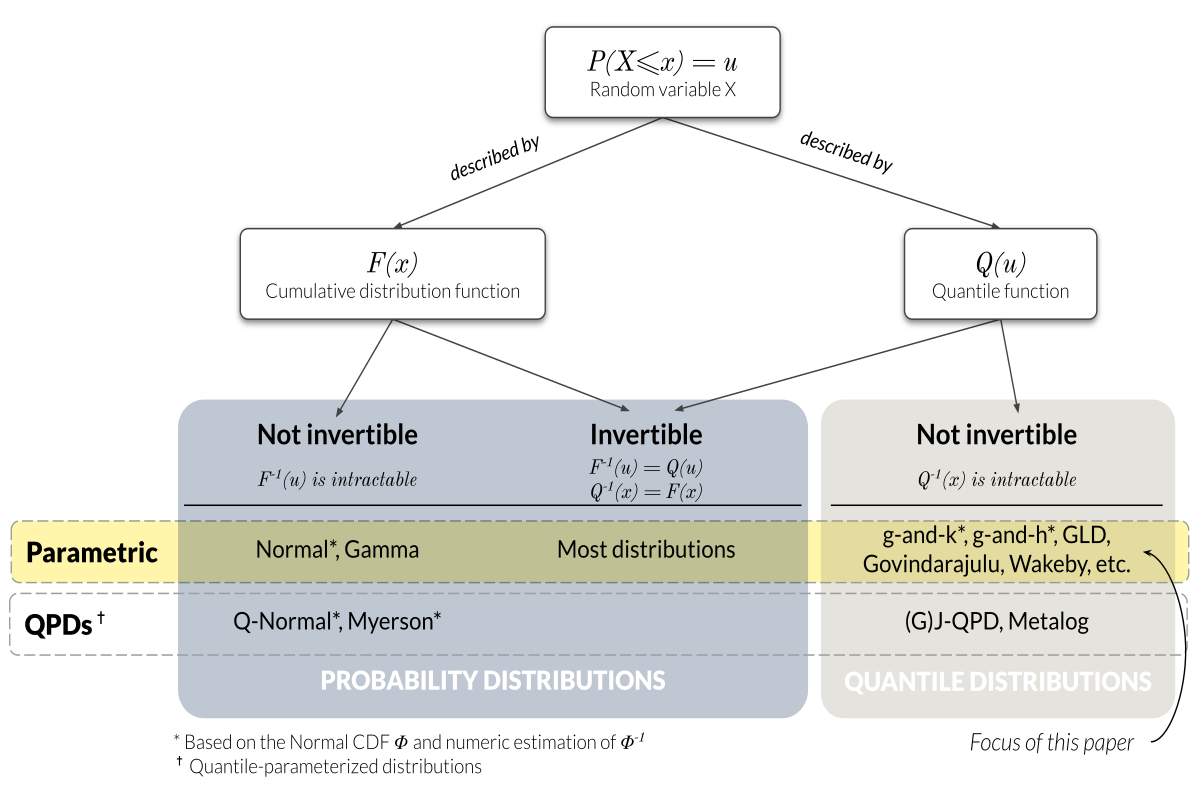
\includegraphics[width=6in]{img/QDs} \caption{Probability distributions, quantile distributions and parameterization by quantiles.}\label{fig:qdist-chart}
\end{figure}

Many specialized distributions have been developed for modeling special kinds of data. These distributions lend themselves naturally as sampling distributions in Bayesian models. Unfortunately some of them are quantile distributions, so Bayesian inference with them up until now was complicated. We suggest some pragmatic simplifications and showcase the example from reliability analysis.

Section 5 discusses the computational aspects of estimating the intermediate CDF values in quantile distributions. We propose a target function and consider several root-finding algorithms which can we applied for numerically inverting the quantile function. The example in this Section shows Bayesian updating using the model with indirect Tukey g-and-h likelihood. We used the Robust Adaptive Metropolis MCMC algorithm by \citet{vihola2012RobustAdaptiveMetropolis} interfaced by the \texttt{fmcmc} package \citep{vegayon2019FmcmcFriendlyMCMC} and a built-in bracketing root-finding algorithm for inverting a quantile function in R.

Section 6 discusses a problem of validating a quantile function, i.e.~checking that the combination of parameters defining the distribution is feasible. We describe the challenges associated with effective checking of quantile function's validity and present the common approaches used for this task. We then propose the use of Chebyshev polynomials \citep{boyd2006ComputingRealRoots} for approximating and root-checking of the quantile density function and discuss the practical aspects of implementing such validation. We illustrate the use of Chebyshev polynomials for proxy root-finding by approximating the quantile density function of the g-and-k distribution and provide custom functions in R implementing the two method of approximation proposed by \citet{boyd2013FindingZerosUnivariate}.

We conclude the paper by discussion and summary of the results in Section 7.

\hypertarget{distribution-specification}{%
\section{Distribution specification}\label{distribution-specification}}

\begin {quotation}
The exact shape doesn't matter \\ 
-- Dodo in Alice's Adventures in Wonderland by Lewis Carroll 
\end{quotation}

Let \(X\) be a continuous random variable. It can be expressed via the distribution function, also known as the \emph{cumulative distribution function} (CDF):

\[
F_X(x | \theta)=Pr(X \leq x | \theta), \quad \theta \in \mathcal A \subset \mathbb R
\]

Alternative way of describing the random variable \(X\) is via the \emph{quantile function} (QF).

\[
Q_X(u | \theta)=\inf\{u:F_X(x|\theta)\geq u\}, \quad 0 \leq u\leq 1
\]

If \(F_X(x)\) is continuous and non-decreasing over the support of \(X\), then \(Q_X(u|\theta)\) is simply an inverse of \(F_X(x|\theta)\). Therefore, the quantile function is often referred to as the ``inverse CDF'', i.e.~

\[
Q_X(u | \theta)=F_X^{-1}(x|\theta)
\]

Unfortunately, not all CDFs are analytically invertible. A distribution defined by a non-invertible quantile function \(Q_X(u | \theta)\) is called a \emph{quantile distribution} (Figure \ref{fig:qdist-chart}).

The derivative of the CDF is the \emph{probability density function} (PDF) denoted by

\[
f_X(x | \theta)=\frac{dF_X}{dx}
\]

Similarly, the derivative of the QF is the \emph{quantile density function} (QDF) denoted by

\[
q_X(u|\theta)=\frac{dQ_X}{du}, \quad 0 \leq u \leq 1
\]

The reciprocal of the QDF \([q_X(u|\theta)]^{-1}=f(Q_X(u|\theta))\) is referred to as the \emph{density quantile function} \citep{parzen1980DataModelingUsing} or \emph{p-pdf} \citep{gilchrist2000StatisticalModellingQuantile}.

\[
f(Q(u))=\frac{dF(Q(u))}{dQ(u)} = \frac{dF(Q(u))/du}{dQ(u)/du}=\frac{dF(F^{-1}(u))/du}{q(u)}=\frac{du/du}{q(u)}=[q(u)]^{-1}
\]

Following the inverse function theorem \citep{price1984InverseFunctionTheorem}, for a function to be invertible in the neighborhood of a point it should have a continuous non-zero derivative at that point. The derivative of the inverse, then, is equal to the reciprocal of the function's derivative. Formally, if \(dy/dx\) exists and \(dy/dx \neq 0\), then \(dx/dy\) also exists and \(dx/dy=[dy/dx]^{-1}\). Therefore, for a distribution function \(F(x)=u\), if a PDF \(f(x)\) exists and \(f(x)\neq0\), then QDF \(q(u)\) also exists and it is equal to \(q(u)=[f(x)]^{-1}\). In Section 3 of this paper, we rely on the density quantile function (DQF) \([q(u|\theta)]^{-1}\) to define the likelihood in a Bayesian model based on the quantile distribution. We call this method of specifying the likelihood ``indirect'', as it is using the CDF value \(u\), representing the observable \(x\) (given the parameter \(\theta\)), and not the observable \(x\) directly.

Even though quantile distributions lack the closed-form CDF \(F_X(x|\theta)\), in most cases, the CDF values can be approximated by numerically inverting the \(Q_X(u|\theta)\). We denote the numerically inverted quantile function as \(\widehat{Q}^{-1}_X(x|\theta)\) or \(\widehat{F}_X(x|\theta)\). The inverse of a quantile function \(Q(u|\theta)\) at point \(u\), corresponding to the observation \(x\), is obtained by minimizing the difference between the actual observation \(x\) and \(Q_X(u|\theta)\) by iteratively refining the CDF value \(u\). The details of the numerical inversion algorithms are discussed in Section 4.

Statistical methods utilizing QF and QDF were pioneered by the seminal work of \citet{parzen1979NonparametricStatisticalData}, although a few years prior to that \citet{tukey1965WhichPartSample} discussed these functions referring to them as the ``representing function'' and the ``sparsity index'', respectively. Today the research area of quantile distributions is an active field of interest for many scientists. The most popular quantile ditributions covered in the literature are Tukey's g-and-k and a related g-and-h distribution \citep{haynes2005BayesianEstimationGandk, jacob2017LikelihoodCalculationGandk, prangle2017GkPackageGandk, rayner2002NumericalMaximumLikelihood}, Tukey's Generalized Lambda Distribution, known as GLD \citep{aldeni2017FamiliesDistributionsArising, chalabi2012FlexibleDistributionModeling, dedduwakumara2021EfficientEstimatorParameters, fournier2007EstimatingParametersGeneralizeda, freimer1988StudyGeneralizedTukey}, Wakeby distribution \citep{rahman2015ApplicabilityWakebyDistribution} and Govindarajulu distribution \citep{nair2012GovindarajuluDistributionProperties, nair2013QuantileBasedReliabilityAnalysis}. Although in this paper we focus on the parametric quantile distributions, the quantile distributions parameterized by the quantile-probability pairs (``quantile-parametrized'' quantile distributions) are also worth a mention, most notably the Johnson QPD (J-QPD) and its generalization \citep{hadlock2017JohnsonQuantileParameterizedDistributions, hadlock2019GeneralizedJohnsonQuantileParameterized}, as well as the metalog distribution \citep{keelin2016MetalogDistributions, keelin2011QuantileParameterizedDistributions}. These distributions play an important role in representing expert beliefs about the variables, parameters or quantities of interest, although they don't lend themselves easily as sampling distributions due to the special features of their parameterization.

\hypertarget{bayesian-inference-for-quantile-functions}{%
\section{Bayesian inference for quantile functions}\label{bayesian-inference-for-quantile-functions}}

\begin{quotation}
You're not shooting the bullet, you're catching it.\\
-- Laura in TENET by Christopher Nolan
\end{quotation}

The first application of Bayesian inference for quantile distributions was proposed by \citet{parzen2004QuantileProbabilityStatistical}, who outlined the method of approximate Bayesian inference using the rejection sampling with the comparison density function \citep[see sections 21-24 in][]{parzen2004QuantileProbabilityStatistical}. In the recent years, many more applications of the approximate Bayesian computation (ABC) to the models defined by the quantile distributions appeared in the literature \citetext{\citealp{allingham2009BayesianEstimationQuantile}; \citealp{drovandi2011LikelihoodfreeBayesianEstimation}; \citealp{dunson2005ApproximateBayesianInference}; \citealp{mcvinish2012ImprovingABCQuantile}; \citealp[and][]{smithson2017CDFquantileDistributionsModellinga}}. ABC methods normally do not require computation of the likelihood, which in case of quantile distributions is convenient, as they lack an explicit CDF and PDF. The few Bayesian applications of quantile distributions involving computation of the likelihood found in the literature, rely on the numerical methods for inverting the quantile function and integrating it into the PDF \citep{prangle2017GkPackageGandk, bernton2019ApproximateBayesianComputation}. The Bayesian inference proposed in this paper makes numeric integration unnecessary, as the density calculation becomes available in closed form using the quantile density function.

\hypertarget{direct-and-indirect-likelihood}{%
\subsection{Direct and indirect likelihood}\label{direct-and-indirect-likelihood}}

In their recent work \citet{nair2020BayesianInferenceQuantile} showed that the traditional Bayesian inference formula can be equivalently restated using the substitutions involving the quantile function. Assume that the prior information about the parameter \(\theta\) can be summarized by the prior distribution of \(f(\theta)\). Then, given a random sample of \(\underline x=\{x_1, x_2, \dots x_n\}\), the posterior distribution of \(\theta\) can be expressed as:

\[
f(\theta|\underline{x}) \propto \mathcal{L}(\theta;\underline{x})f(\theta)
\label{eq:bayespdfeq}
\]

where \(f(\theta|\underline{x})\) is the posterior distribution of \(\theta\) after having observed the sample \(\underline{x}\), \(f(\theta)\) is the prior distribution of \(\theta\), and \(\mathcal{L}(\theta;x)=\prod_{i=1}^{n}f(x_i|\theta)\) is the likelihood. We refer to this form of likelihood as ``direct'', because the observables \(x\) are directly used as input to the likelihood function.

Given the random sample of \(\underline x\), we can use the QF to compute \(\underline{Q}=\{Q_1(u_1), Q_2(u_2), \dots Q_n(u_n)|\theta\}\), such that \(u_i=F(x_i|\theta), i=1\dots n\). The CDF values \(u_i\), which we try to avoid calling ``probabilities'' in the context of indirect likelihood and rather denote by \(\underline u|\theta\), can be thought of as degenerate random variables, because they are fully determined given the observables \(\underline{x}\) and parameter \(\theta\). Since \(Q(u_i|\theta)=x_i\) we can substitute \(\underline Q\) for \(\underline x\). Then the Bayesian inference formula \eqref{eq:bayespdfeq} becomes:

\[
f(\theta|\underline{Q}) \propto \mathcal{L}(\theta;\underline{Q})f(\theta)
\label{eq:bayesdqfeq}
\]

We refer to the likelihood \(\mathcal{L}(\theta;\underline{Q})=\prod_{i=1}^{n} f(Q(u_i|\theta))=\prod_{i=1}^n[q(u_i|\theta)]^{-1}\) as ``indirect'', because it relies on computing of intermediate CDF values \(u_i=F(x_i|\theta), i=1\dots n\), which are then supplied to the quantile function \(Q(\underline u|\theta)\).

As we have shown, the two forms of likelihood \(\mathcal{L}(\theta;\underline{Q})\) and \(\mathcal{L}(\theta;\underline{x})\) are proportional to each other. Therefore, following the likelihood principle, the posterior beliefs about \(\theta\) are independent of the form of the likelihood function used.

Since the likelihood in the Equation \eqref{eq:bayesdqfeq} is expressed in terms of \(\underline {Q}=Q(\underline{u}|\theta)\), additional transformation is required to arrive at \(\underline{u}=F(\underline{x}|\theta)\). In case the closed form of the CDF \(F(\underline x|\theta)\) is not available, the numeric approximation of \(\widehat{Q}^{-1}(\underline{x}|\theta)\) may be used. We discuss the details of the numerical approximation of the inverse quantile function in Section 5 of this paper.

\hypertarget{example}{%
\subsubsection{Example}\label{example}}

To illustrate the equivalence of the two ways of specifying likelihood in Bayesian models, we use the example from \citet{klugman2004LossModelsData}\footnote{Example 16.17 on p.544} regarding the distribution of the claim amounts (referred to hereinafter, as the Claims Example).

\citet{klugman2004LossModelsData} model the claim amounts using exponential distribution with the mean of \(1/\lambda\), where parameter \(\lambda\) is following the gamma distribution with the shape \(\alpha=4\) and the scale \(\beta=0.001\). Given three observations of the claim amounts \(\underline x=\) 100, 950 and 450, we sample from the posterior distribution of the parameter \(\lambda\) using the HMC algorithm in Stan \citep{standevelopmentteam2021RStanInterfaceStan}. Since gamma prior is conjugate to the exponential sampling distribution \citep{pratt1995IntroductionStatisticalDecision} we can verify the distribution of the posterior draws using the analytic solution.

Exponential distribution function \(F(x)\) and the probability density function \(f(x)\) are given by

\[
\begin{gathered}
F(x)=1-e^{-\lambda x} \\ 
f(x)=\lambda e^{-\lambda x}
\end{gathered}
\]

where \(\lambda>0\) and \(x\in[0,\infty)\).

Exponential quantile function \(Q(u)\) and quantile density function \(q(u)\) are

\[
\begin{gathered}
Q(u)=-\frac{\ln(1-u)}{\lambda}\\ 
q(u)=\frac{dQ(u)}{du}=\frac{1}{\lambda(1-u)}
\end{gathered}
\]

where \(\lambda>0\) and \(u=F(x), u \in [0,1]\)

Since gamma prior is conjugate to the exponential sampling distribution, the posterior density of \(\lambda\) can be described by

\[
f(\lambda|\underline{x})=\text{Gamma}(\lambda| \alpha+N, \beta+\sum \underline{x} )
\]

where \(\alpha\) and \(\beta\) are the parameters of gamma distribution and \(\underline{x}=\{x_1, x_2, \dots x_N\}\) is the sample of observations of size \(N\).

Table \ref{tab:gexp-likelihood-tab} and Figure \ref{fig:gexp-likelihood-graphs} present the posterior distribution of \(\theta\) from the two Gamma-Exponential models: one with a direct and another one with an indirect likelihood, along with the posterior from the conjugate model. Stan programs for the corresponding examples are provided in the Supplementary Material.

\begin{table}[!h]

\caption{\label{tab:gexp-likelihood-tab}Posterior sample comparison for the models}
\centering
\begin{tabular}[t]{lrrrrr}
\toprule
variable & mean & median & q5 & q95 & rhat\\
\midrule
lambda (direct likelihood) & 0.0028324 & 0.0026905 & 0.0013352 & 0.0047949 & 1.000157\\
lambda (indirect likelihood) & 0.0028291 & 0.0026787 & 0.0013695 & 0.0047937 & 1.000506\\
\bottomrule
\end{tabular}
\end{table}

\begin{figure}

{\centering 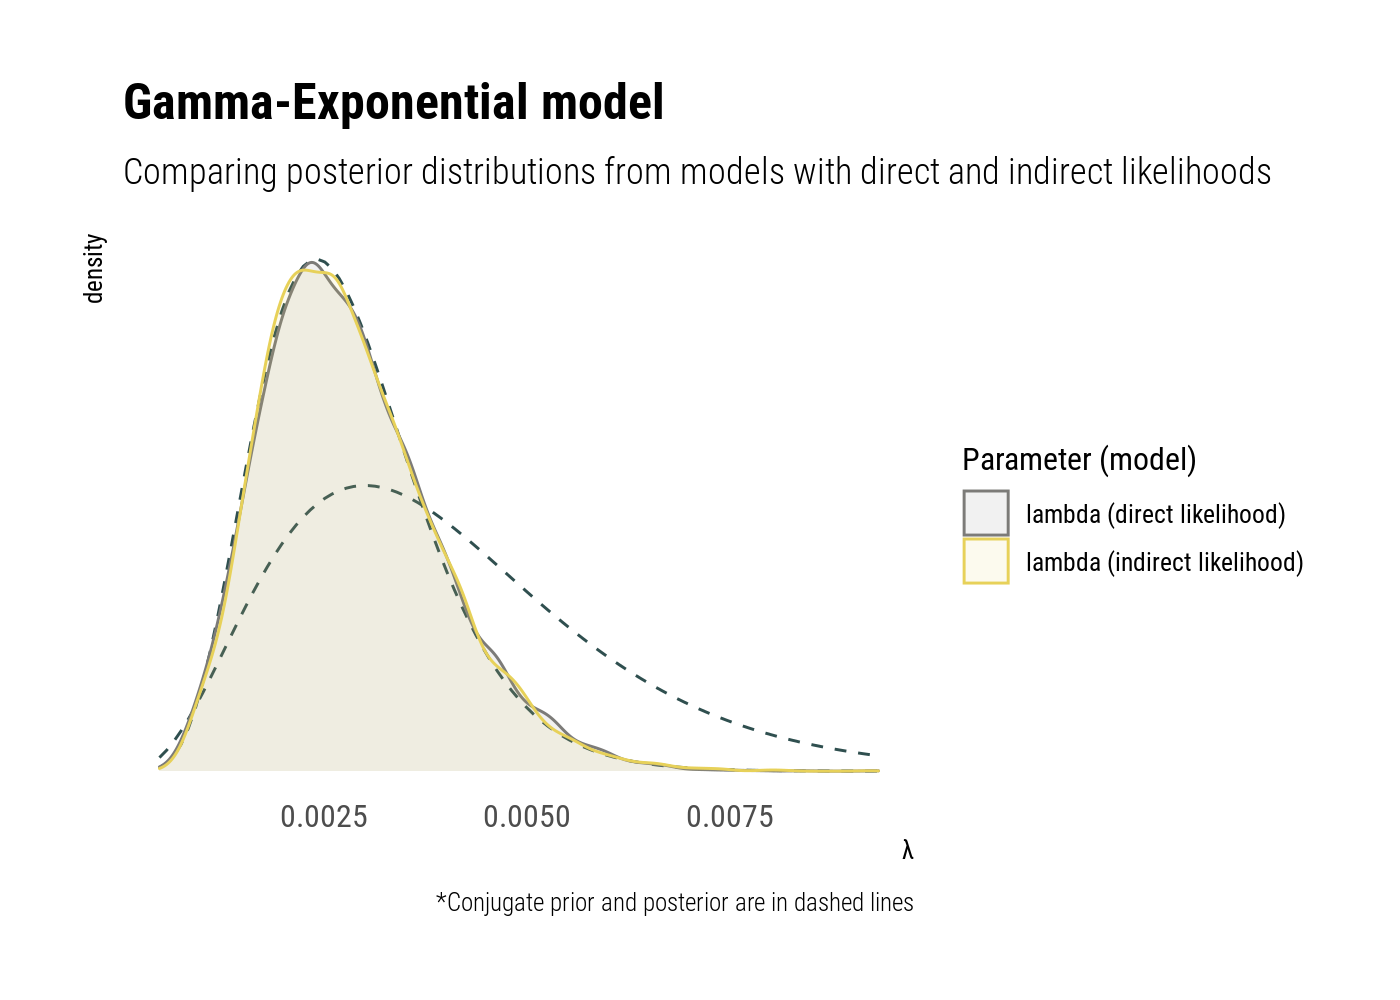
\includegraphics[width=0.5\linewidth]{ilbm_article_files/figure-latex/gexp-likelihood-graphs-1} 

}

\caption{Summary of the posterior samples from the gamma-exponential model with direct and indirect likelihood}\label{fig:gexp-likelihood-graphs}
\end{figure}

As we can observe the posterior distributions of parameter \(\lambda\) from the two models are equivalent match the analytic solution from the conjugate model within the sampling error.

\hypertarget{direct-and-indirect-prior}{%
\subsection{Direct and indirect prior}\label{direct-and-indirect-prior}}

Bayesian inference formula can also be restated using the quantile form of the prior. Assume that the prior distribution of \(\theta\) can be described using the invertible distribution \(F_\Theta(\theta)=v\), so that \(Q(v)=\theta\). Substituting the quantile values \(Q(v)\) for values of \(\theta\), prior beliefs about the parameter(s) of the sampling distribution can be expressed indirectly using the distribution of the quantile values corresponding to the CDF value \(v\), given hyperparameter(s) of the prior distribution \eqref{eq:bayesdqfdqfeq}.

\[
\begin{gathered}\;
f(Q(v)|\underline{x}) \propto \mathcal{L}(Q(v);\underline{x})f(Q(v)) \\
[q(v|\underline{x})]^{-1} \propto \mathcal{L}(Q(v);\underline{x})[q(v)]^{-1}
\end{gathered}
\label{eq:bayesdqfdqfeq}
\]

where \([q(v|\underline{x})]^{-1}\) is the indirect form of the quantile posterior, \([q(v)]^{-1}\) is the indirect form of quantile prior and \(\mathcal{L}(Q(v);\underline{x})\) is the direct likelihood, relying on the non-linear parameter transformation \(\theta=Q(v)\). The likelihood with such parameter transformation requires a Jacobian adjustment which is equal to the absolute derivative of the transform, i.e.~\(J(Q(v))=|dQ(v)/dv|=|q(v)|\). We refer to such formulation of the prior as the \emph{indirect prior} because relies on the quantile transformation \(\theta=Q(v)\) and therefore its density is expressed in the quantile form \([q(v)]^{-1}\).

Of course indirect prior can also be used in combination with indirect likelihood, since, as we showed previously, the two of them lead to the same posterior beliefs about the parameter \(\theta\) and, consequently, \(v\). In such case, neither prior nor likelihood would require the existence of the closed-form PDF and, therefore, both of them can be represented by quantile distributions.

Provided that the \(Q(v)\) is a valid (non-decreasing) quantile function, meaning that \(q(v)\) is non-negative on \(v \in [0,1]\), the quantile density terms representing the prior and the Jacobian adjustment can be dropped as they are reciprocal to each other.

\[ 
\begin{gathered}\;
[q(v|\underline{x})]^{-1} \propto \mathcal{L}(Q(v);\underline{x})[q(v)]^{-1}|q(v)| \\
[q(v|\underline{x})]^{-1} \propto \mathcal{L}(Q(v);\underline{x})
\end{gathered}
\label{eq:bayesidqfeq}
\]

where \([q(v|\underline{x})]^{-1}\) is the quantile form of the posterior, and the prior belief about the parameter \(\theta\) is represented by the quantile function transform of the parameter \(v \in [0,1]\) (given the relevant hyperparameters), such that \(Q(v)=\theta\). This formulation is commonly known as the ``inverse transform'' because it relies on the QF (inverse CDF) transformation of the unit parameter \(v\).

\hypertarget{example-1}{%
\subsubsection{Example}\label{example-1}}

In the Claims Example the prior belief about the distribution of the exponential parameter \(\lambda\) was represented by the Gamma distribution, which is, unfortunately not easily invertible (Figure \ref{fig:qdist-chart}). In order to illustrate the indirect specification of the prior, we switch to the Rayleigh prior represent the expert's beliefs about the exponential parameter \(\lambda\). The shape of the new prior \(Rayleigh(0.003)\) is comparable to the gamma prior \(Gamma(4,0.001)\) used previously.

\begin{figure}

{\centering 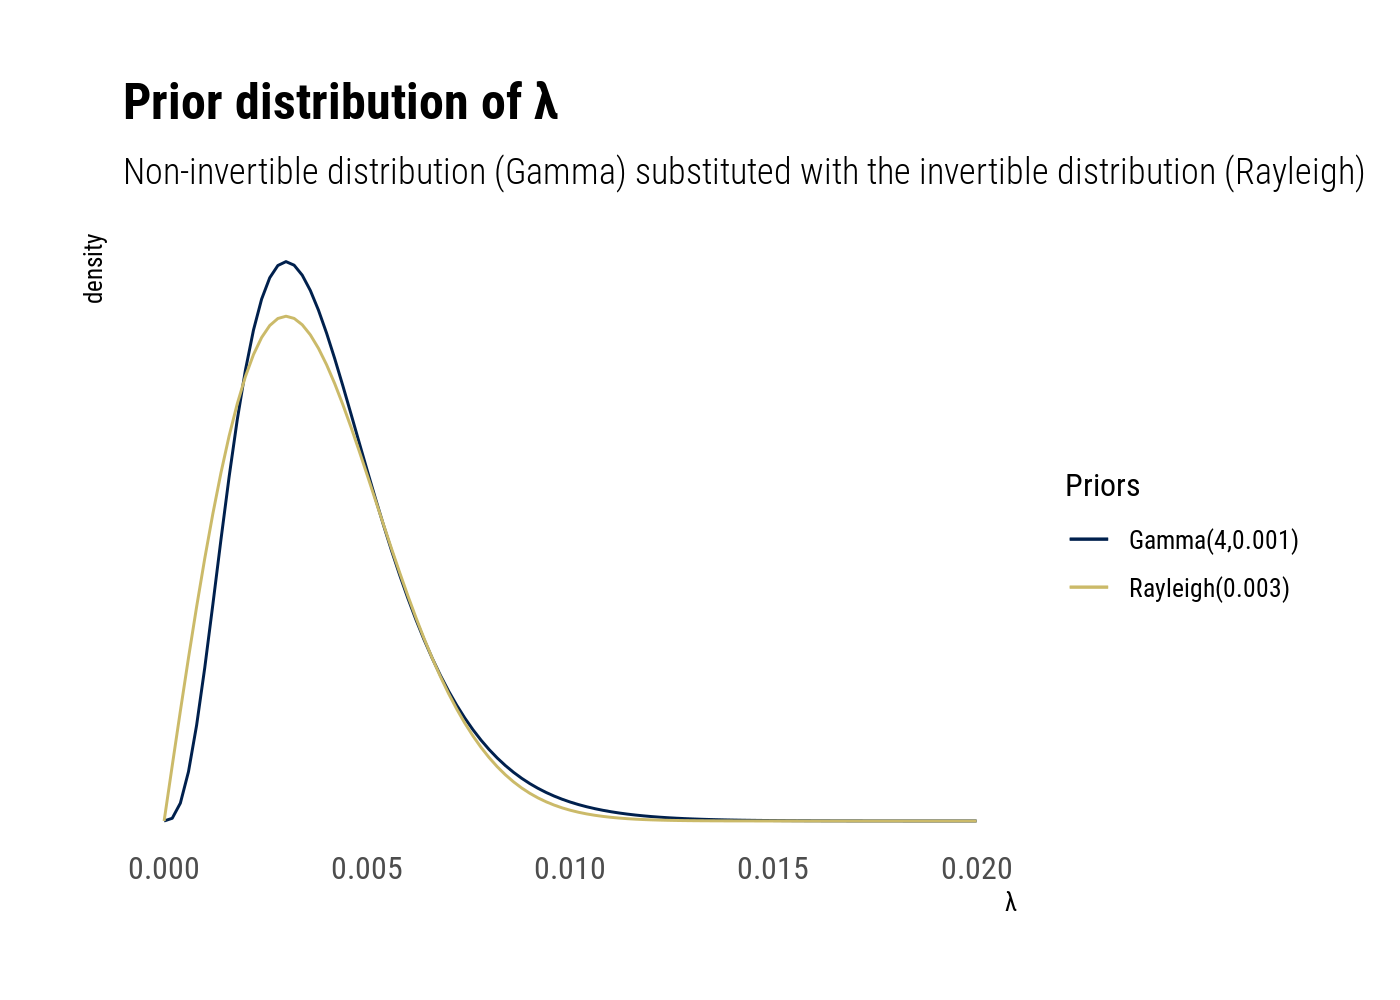
\includegraphics[width=0.5\linewidth]{ilbm_article_files/figure-latex/gamma-ray-prior-graph-1} 

}

\caption{Prior distribution of the rate parameter of Exponentail distribution}\label{fig:gamma-ray-prior-graph}
\end{figure}

Rayleigh distribution function \(F(x)\) and probability density function \(f(x)\) are:

\[ 
\begin{gathered}\;
F(x|\sigma) = 1-\exp(-x^2/(2\sigma^2)) \\ 
f(x|\sigma) = \frac{x}{\sigma^2}\exp(-x^2/(2\sigma^2))
\end{gathered}
\]

where \(\sigma>0\) is Rayleigh scale parameter.

Rayleigh quantile function \(Q(p)\) and quantile density function \(q(p)\) are:

\[
\begin{gathered}\;
Q(p|\sigma)=\sigma\sqrt{-2\ln(1-p)} \\ 
q(p|\sigma)=\frac{\sigma}{\sqrt{2}\sqrt{-\ln(1-p)}(1-p)}
\end{gathered}
\]

where \(\sigma>0\) and \(p \in [0,1]\).

\begin{table}[!h]

\caption{\label{tab:rexp-prior-lik-tab}Summary of the posterior samples from the Rayleigh-Exponential model with direct and indirect prior and likelihood}
\centering
\begin{tabular}[t]{lrrrrr}
\toprule
variable & mean & median & q5 & q95 & rhat\\
\midrule
lambda (direct prior, direct likelihood) & 0.0026969 & 0.0025534 & 0.0011192 & 0.0047638 & 1.000932\\
lambda (direct prior, indirect likelihood) & 0.0026911 & 0.0025490 & 0.0011319 & 0.0047732 & 1.001204\\
lambda (indirect prior, direct likelihood) & 0.0027010 & 0.0025755 & 0.0011266 & 0.0047007 & 1.000218\\
lambda (indirect prior, indirect likelihood) & 0.0027172 & 0.0025843 & 0.0011114 & 0.0047745 & 1.000886\\
\bottomrule
\end{tabular}
\end{table}

Table \ref{tab:rexp-prior-lik-tab} and Figure \ref{fig:rexp-prior-lik-graphs} compare the posterior distribution of \(\theta\) from the gamma-exponential model with direct and indirect likelihood. Stan programs for corresponding examples are provided in the Supplementary Material.

\begin{figure}

{\centering 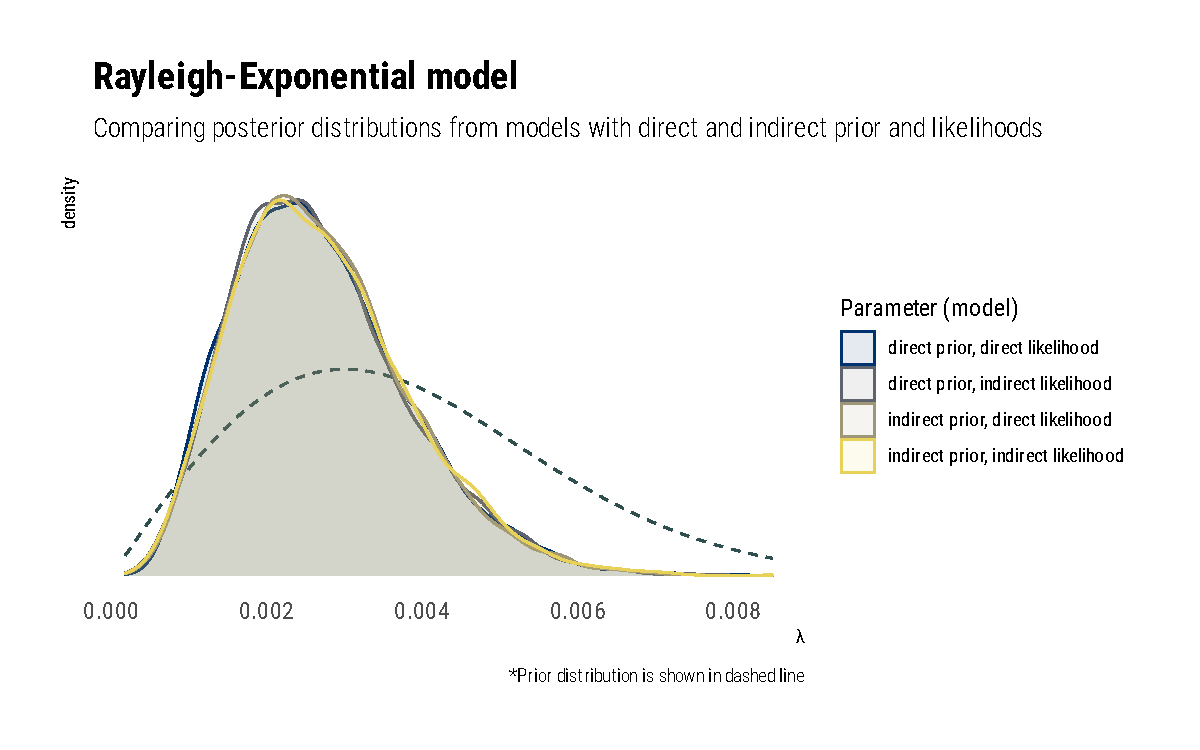
\includegraphics[width=0.5\linewidth]{ilbm_article_files/figure-latex/rexp-prior-lik-graphs-1} 

}

\caption{Distribution of the posterior samples from the Rayleigh-Exponential model with direct and indirect prior and likelihood}\label{fig:rexp-prior-lik-graphs}
\end{figure}

\hypertarget{specialized-quantile-sampling-distributions}{%
\section{Specialized quantile sampling distributions}\label{specialized-quantile-sampling-distributions}}

Indirect likelihood would be an curious, yet impractical method of performing Bayesian inference if there weren't instances and areas of application, where quantile sampling distributions are essential. Many quantile distributions have been developed with particular application in mind, offering some unique advantages, not easily replicateable with the conventional density-defined distributions.

\citet{nair2020BayesianInferenceQuantile} provide an example from \citet{aarset1987HowIdentifyBathtub} of time to failure of 50 devices put on the life test at time 0. The data clearly represents an instance of a process with a bathtub-shaped hazard rate (see Figure \ref{fig:bathtub-hist}). Lifetime reliability data are often modeled using specialized distributions \citep{nadarajah2009BathtubshapedFailureRate} or the three- (or two-) component mixtures. \citet{nair2020BayesianInferenceQuantile} used the maximum likelihood method to estimate the parameter \(\gamma\) of the Govindarajulu distribution \citep{nair2012GovindarajuluDistributionProperties} described by the generalized exponential prior \citep{gupta2007GeneralizedExponentialDistribution}. We reuse the \citet{aarset1987HowIdentifyBathtub} example and estimate the full posterior distribution of both parameters of the Govindarajulu sampling distribution.

\begin{figure}

{\centering 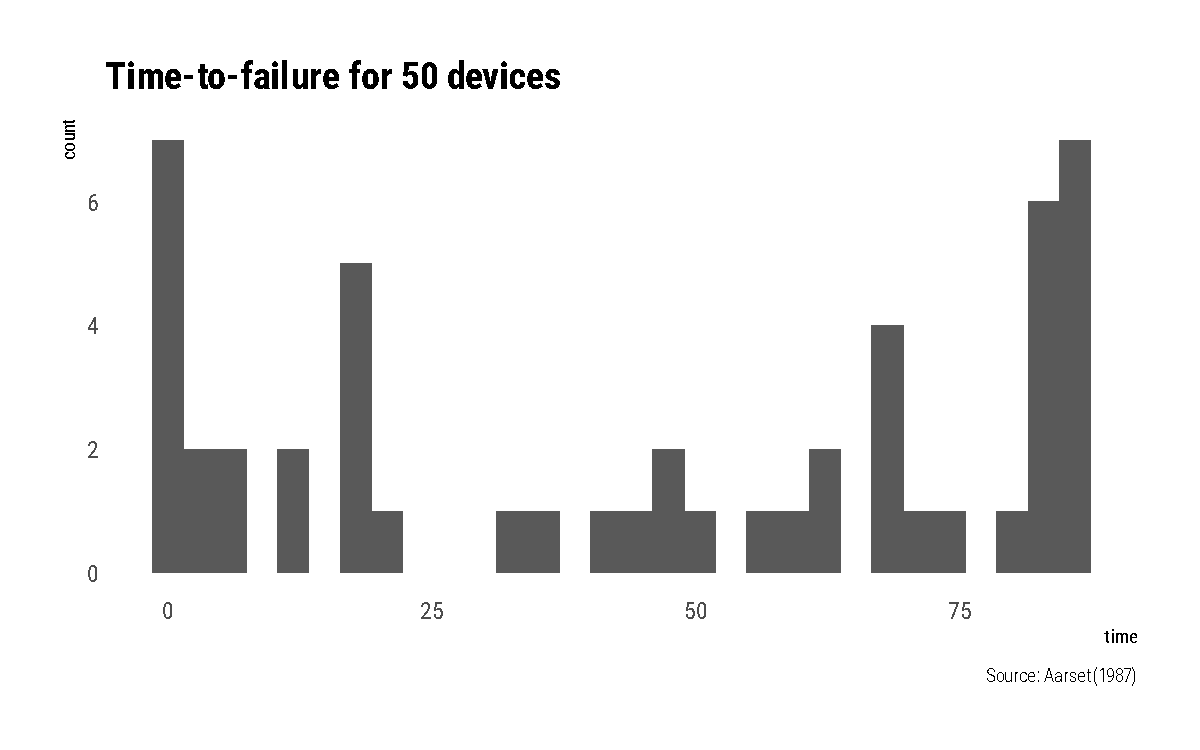
\includegraphics[width=0.5\linewidth]{ilbm_article_files/figure-latex/bathtub-hist-1} 

}

\caption{Histogram of the time to failure data}\label{fig:bathtub-hist}
\end{figure}

Govindarajulu distribution defined by the quantile function has the following QF and QDF:

\[
\begin{gathered}\;
Q_X(u)=\sigma\gamma u^\gamma(1+\gamma^{-1}-u)\\
q_x(u)=Ku^{\gamma-1}(1-u)
\end{gathered}
\]
where \(K=\sigma\gamma(\gamma+1)\), and \(\gamma>0\).

The Govindarajulu distribution has support on \((Q(0), Q(1))=(0, \sigma)\)\footnote{For definition of the distribution with shifted support see \citet{nair2012GovindarajuluDistributionProperties}}.

Generalized exponential distribution has the following CDF and PDF:

\[
\begin{gathered}\;
F(x)=(1-e^{-\lambda x})^\alpha \\
f(x)=\alpha\lambda(1-e^{-\lambda x})^{\alpha-1}e^{-\lambda x}
\end{gathered}
\]

where \(x, \alpha, \lambda>0\).

We used generalized exponential prior for the parameter \(\gamma\) of Govindarajulu distribution with hyperparameters \(\alpha\) = 5 and \(\lambda\) = 1.

We reuse the same generalized exponential prior as proposed in \citep{nair2020BayesianInferenceQuantile}. Generalized exponential QF is then:

\[
Q(u)=-\frac{1}{\lambda}ln(1-u^{1/\alpha})
\]

The parameter \(\sigma\) of the Govindarajulu distribution can not be lower than the maximum of the observed times-to-failure. We defined exponential prior with \(\lambda\) = 1 and varying lower bound corresponding to the highest time to failure, in our example equal to 86. The Jacobian for adding a constant to the sampled parameter \(\sigma\), although required, is equal to one, so there will be no impact on the log density, as the shifting transform produces a Jacobian derivative matrix with a unit determinant.

\begin{figure}

{\centering 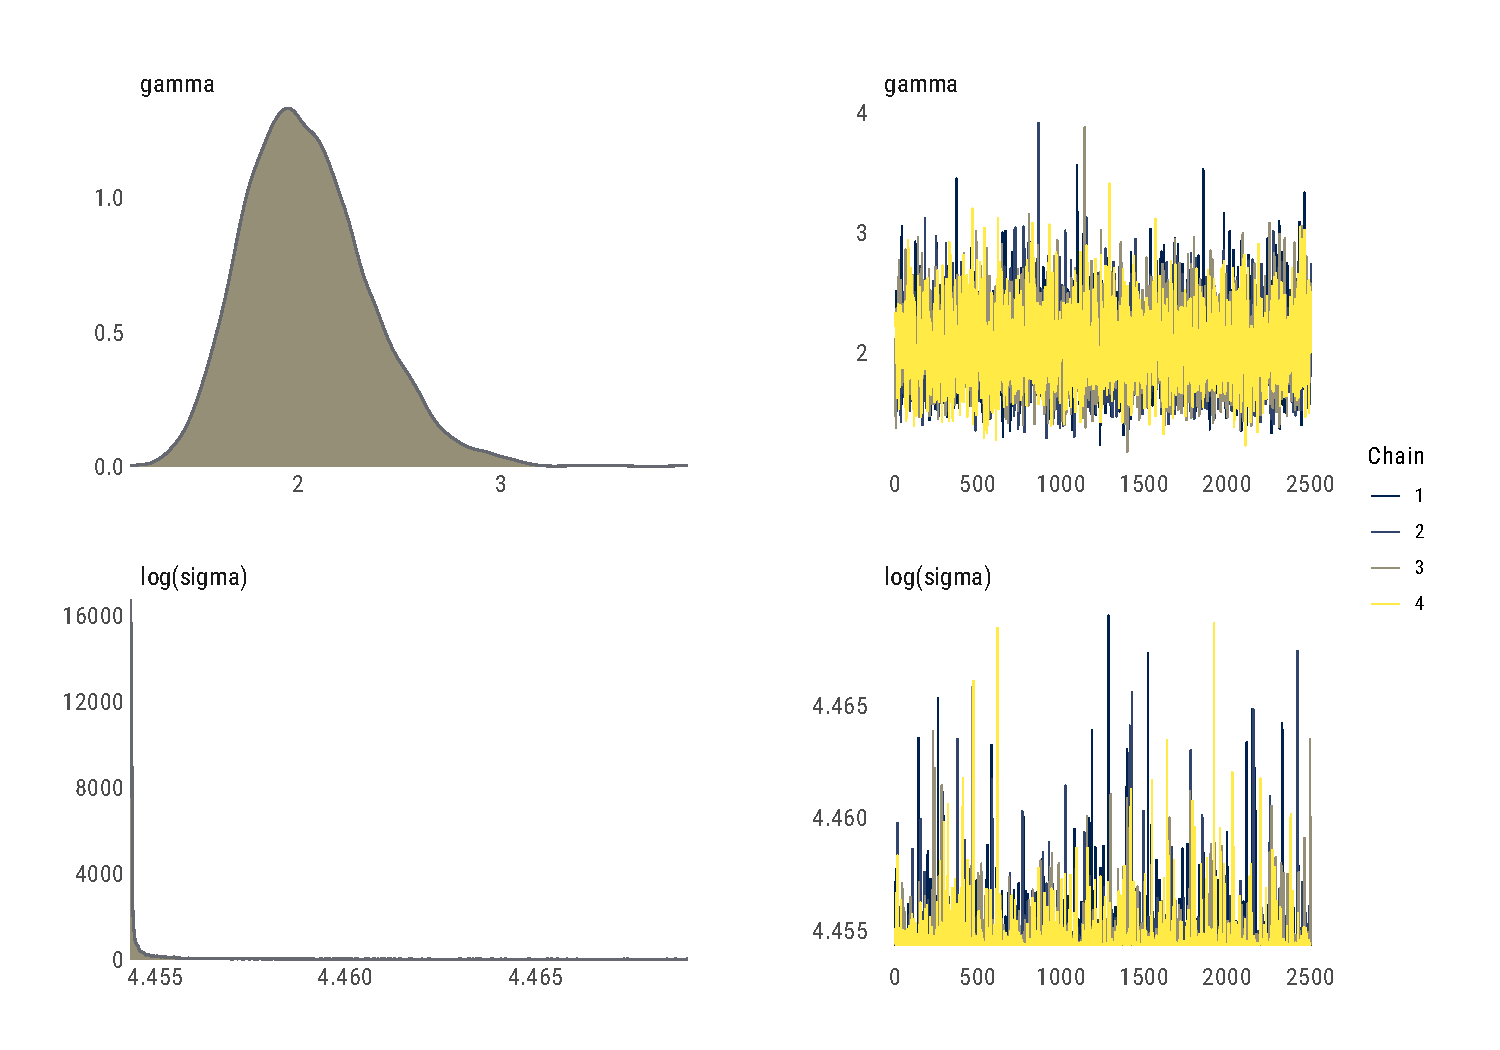
\includegraphics[width=0.8\linewidth]{ilbm_article_files/figure-latex/unnamed-chunk-6-1} 

}

\caption{Posterior distribution and traceplot for parameters of GenExp-Govindarajulu model}\label{fig:unnamed-chunk-6}
\end{figure}

\hypertarget{numerical-inverting-of-quantile-function}{%
\section{Numerical inverting of quantile function}\label{numerical-inverting-of-quantile-function}}

\begin{quotation}
One of the bullets are like us, traveling forward through time. The other runs backwards.
-- Laura in TENET by Christopher Nolan
\end{quotation}

The core element of the indirect likelihood method is the use of the intermediate CDF values \(\underline{u}\), corresponding to the observables \(\underline{x}\) given the parameter \(\theta\). These values can either be found analytically, as \(Q^{-1}(x)=F(x)\) for invertible probability distributions, or, otherwise, numerically via root-finding algorthm, as \(\widehat{Q}^{-1}_X(x)=\widehat{F}_X(x)\) e.g in case of quantile distributions (Figure \ref{fig:qdist-chart}).

The problem of inverting a quantile function is tantamount to finding the root of a target function

\[
Z(u|\theta)=[x-Q_X(u|\theta)]
\]

where \(x\) is a known observation, \(\theta\) is the parameter value, and \(u|\theta\) is the CDF value \(u\), such that \(Z(u|\theta)=0\). Given that the \(Q(u|\theta)\) is a non-decreasing function and \(x\) is fixed observable value, the target function \(Z(u|\theta)\) is non-increasing. In principle, the choice of the algorithms for finding the zeroes of a target function \(Z\) includes two broad groups of methods: \emph{bracketing} and \emph{gradient} \citep{atkinson2008IntroductionNumericalAnalysis, burden2011NumericalAnalysis}.

The bracketing methods, such as bisection, secant, Lagrange polynomial and Brent method, require a pair of values around the root, i.e.~two values of \(u^+\) and \(u^-\), such that \(Z(u^+|\theta)>0\) and \(Z(u^-|\theta)<0\). In order for the algorithm to converge faster, the interval \([u^+, u^-]\) needs to be relatively narrow. As \(Q^{-1}(x)=F(x)\) is a non-decreasing function, the interval of CDF values \([u^+, u^-]\) enclosing the true value \(u|\theta\) corresponding to the observable \(x\), can be found by matching the observable \(x\) to the sorted grid of \(K\) quantile values \(Q^{grd}_k=Q_X(u^{grd}_k|\theta), \quad k \in 1..K\), where \(\forall u^{grd}_k, k \in (1\dots K): 0<u^{grd}_k<1, \; u^{grd}_k<u^{grd}_{k+1}\) come from a sorted grid of CDF values. Once \(x\) is matched to the grid of quantiles \(Q^{grd}_k\), the quantile value immediately preceding the observable \(x\) and immediately following it, such that \(Q^{grd}_{m} \leq x \leq Q^{grd}_{m+1}\) can be determined and the corresponding CDF values \(u^{grd}_m\) and \(u^{grd}_{m+1}\) can be returned. The interval formed by these CDF values can be adopted as \([u^+, u^-]\), as it is guaranteed to contain the value of \(u\) corresponding to the root of the target function \(Z(u|\theta)\).

The gradient methods, such as Newton-Rhapson, rely on a single ``initial guess'' value \(u_{(i)}\) and the gradient represented by the derivative of a target function \(Z^\prime(u_{(i)}|\theta)\). Following this method the ``improved'' value \(u^*\) can found as:

\[
u^*\approx u_{(i)} -\frac{Z(u_{(i)})}{Z^\prime(u_{(i)})}
\]

Substituting the target function \(Z\), the Newton-Raphson method for finding the inverse of the quantile function becomes:

\[
u^*\approx u_{(i)}-\frac{x-Q_X(u_{(i)}|\theta)}{d[x-Q_X(u_{(i)}|\theta)]/du_{(i)}}= u_{(i)}+\frac{x-Q_X(u_{(i)}|\theta)}{q_X(u_{(i)}|\theta)}
\]

where \(u_{(i)}\) is the initial value of the probability (the ``CDF value'') \(u\), corresponding to the observation \(x\) given \(\theta\), \(u^*\) is the new (improved) value of \(u_{(i)}\) after an iteration and \(q_X(u_{(i)}|\theta)\) is the QDF of X, which is the first derivative of the QF \(Q_X(u_{(i)}|\theta)\) with respect to the CDF value \(u_{(i)}\). The procedure can be repeated by taking the approximated \(u^*\) as a new initial value \(u_{(i)}\) and recomputing the value of \(u^*\), until \(|Z(u_{(i)})|\theta)|< \epsilon\), where \(\epsilon\) is some small value. Again, for faster convergence it is desirable that the initial guess value \(u_{(i)}\) is as close to the true root as possible. The method has been used in the literature for approximating CDFs of several known quantile distributions \citetext{\citealp[see p.99 in][]{gilchrist2000StatisticalModellingQuantile}; \citealp[p.345 in][]{nair2013QuantileBasedReliabilityAnalysis}}.

The Figure \ref{fig:newton-animation-graph} illustrates the numerical approximation of the CDF value \(u\) corresponding to the observed claim amount equal to \(100\) in the Claims Example, given the sampling distribution \(Exponential(0.002)\). We provide the uninformed guess of 0.5 as pretty ignorant initial value. The algorithm required 4 iterations to arrive at the approximation of the true CDF value of 0.1812692 given the desired tolerance, which for the purposes of this example we set at \(10^{-3}\).

\begin{figure}

{\centering 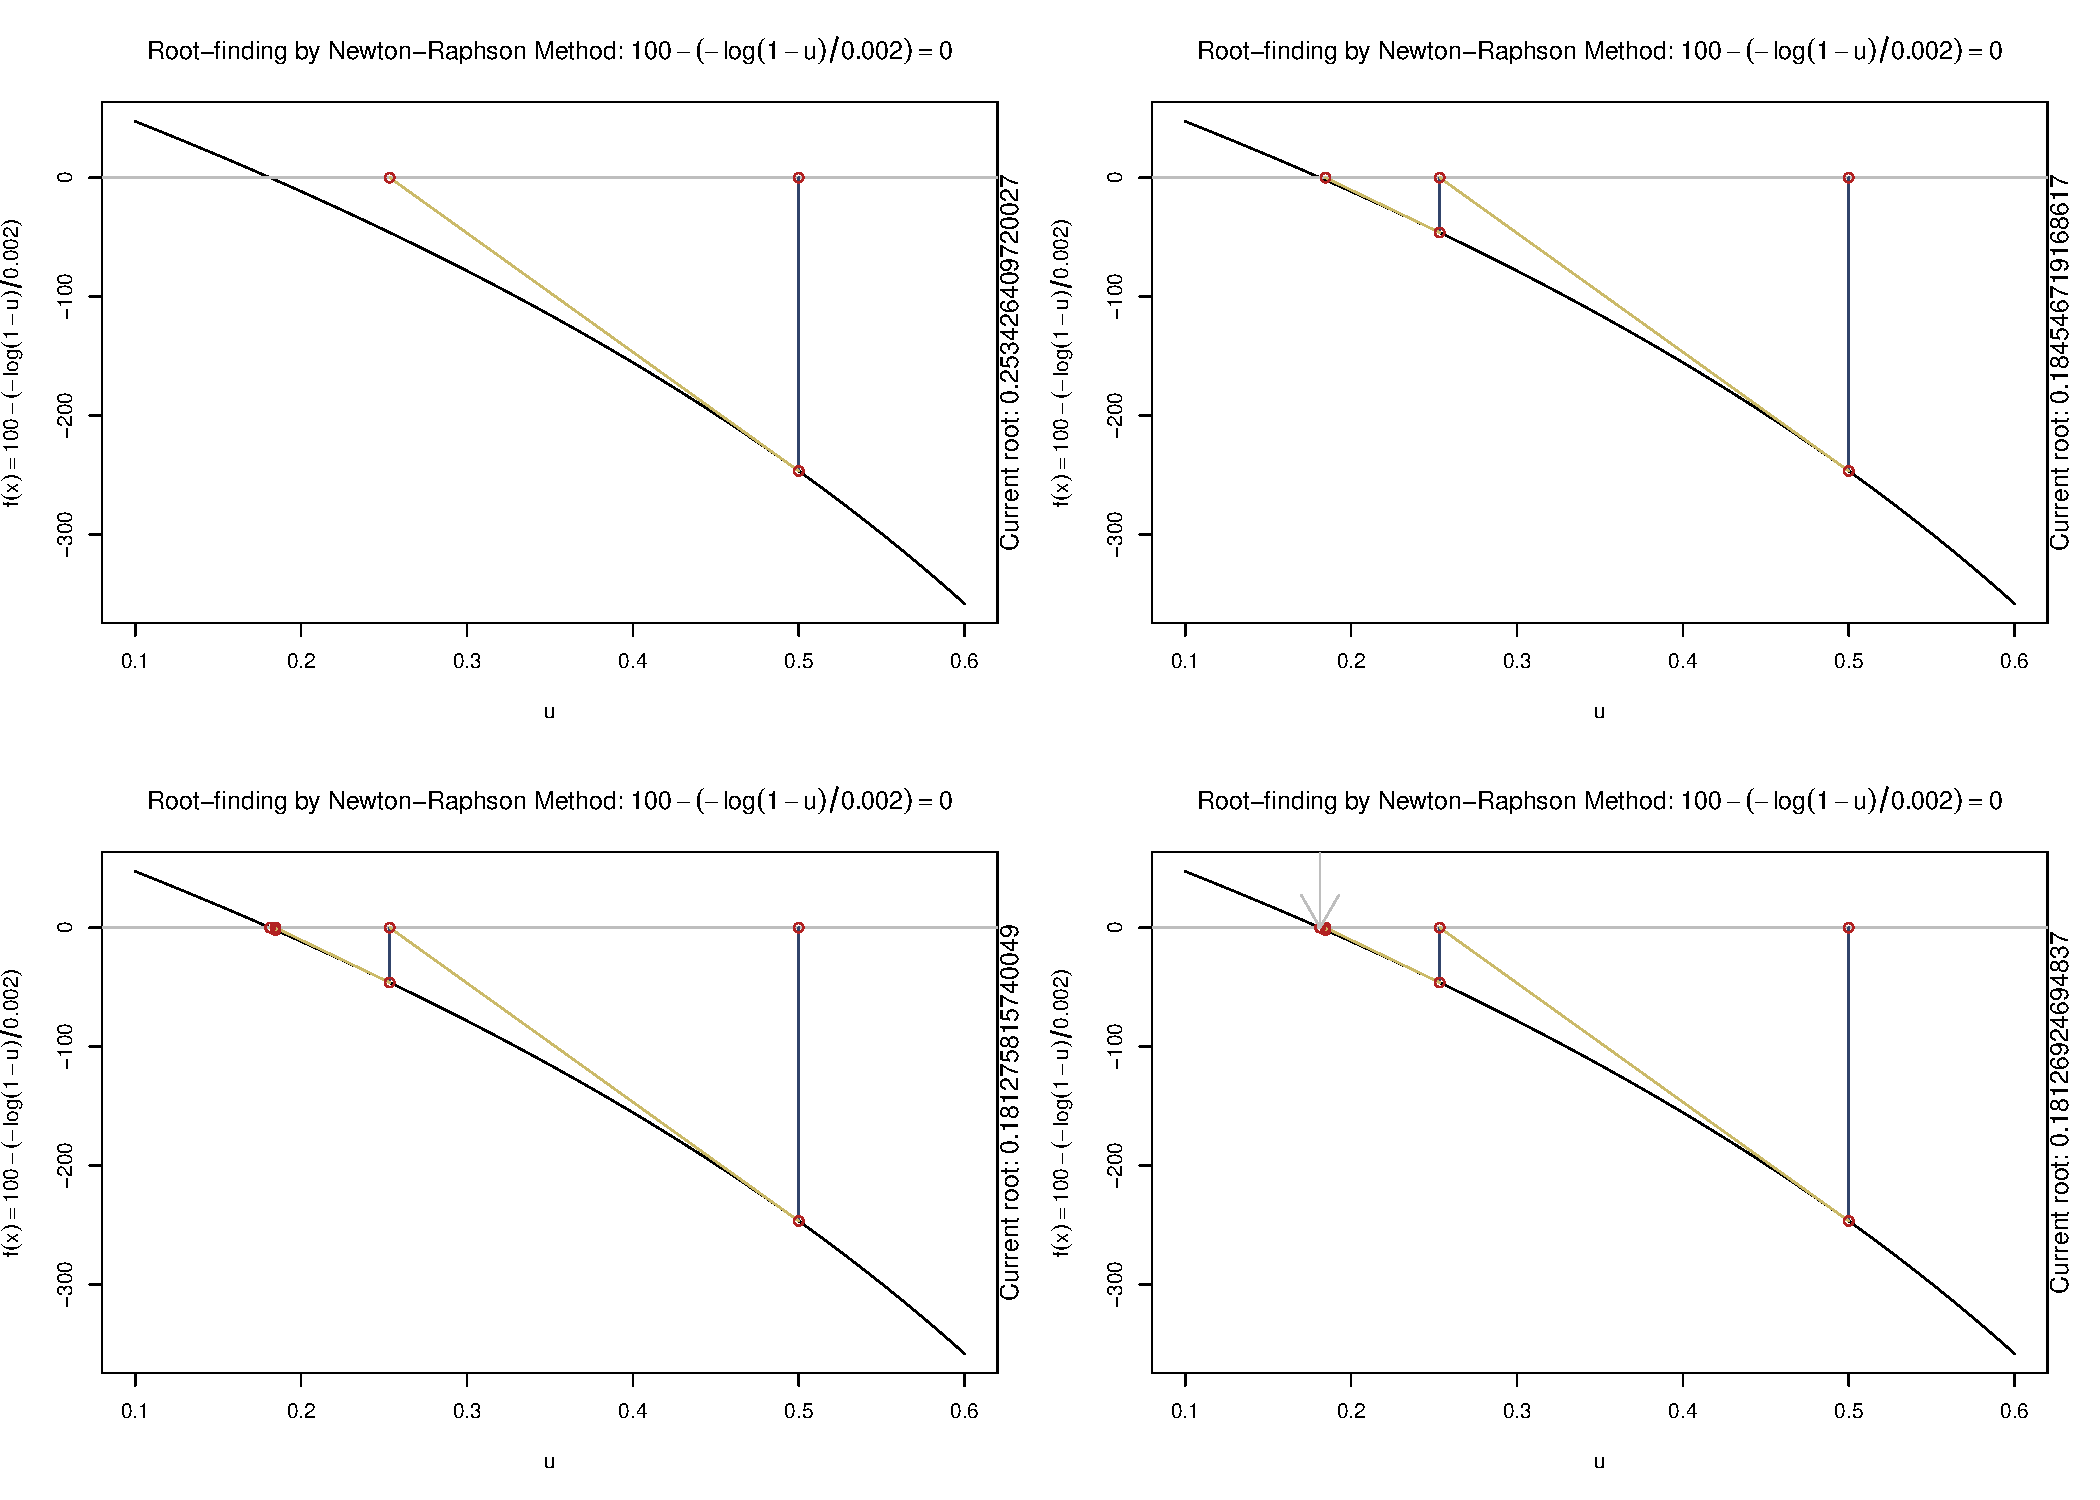
\includegraphics[width=0.5\linewidth]{img/newton-graph} 

}

\caption{Approximating the CDF values in the Exponential model using Newton-Rhapson method}\label{fig:newton-animation-graph}
\end{figure}

There are other methods which can be adapted for finding the zeroes of a function, even though they may be developed for a different purpose. In the absence of other built-in root-finders, inthe previous example utilizing the Givindarajulu likelihood we used Stan's solver, intended for finding the roots of linear systems, to numerically determine the CDF values corresponding to the observable times to failure. Stan's \texttt{algebra\_solver()} is based on the Powell hybrid method, initially developed for finding the local minimum of a function. Powell's hybrid method combines of advantages of the Newton's method with the steepest descent method, which guarantees stable convergence \citep{powell1970HybridMethodNonlinear}.

In this section we illustrate the use of the Brent's root-finding algorithm implemented in R as \texttt{stats::uniroot()} for inverting the quantile function of the Tukey's \emph{g-and-h} distribution \citep{rayner2002NumericalMaximumLikelihood}. Brent's method, also known as the Brent-Dekkert algorithm, combines the features of the bisection and secant methods with the inverse quadratic interpolation.

Tukey's g-and-h distribution is defined by the quantile funciton:

\[
Q_{gnh}(p)=A+Bz[1+C\tanh(gz/2)]\exp(hz^2/2)
\]

where \(z=z(p)=\Phi^{-1}(p|0,1)\) is standard normal quantile function, \(B>0\) and \(h>0\). The parameter \(g\) is responsible for skeweness, i.e.~when \(g<0\) the distribution is skewed left, and when \(g>0\), it is skewed right. The parameter \(h\) is responsible for kurtosis. For all values of kurtosis greater than that of the normal distribution, i.e.~\(h\geq 0\), regardless of value of \(g\), the parameter \(C \leq 0.83\) (approximately) results in a proper distribution. In practice the parameter \(C\) is often set to 0.8 \citep{prangle2017GkPackageGandk}.

g-and-h distribution QDF can be obtained by differentiating the QF with respect to the probability \(p\) using the chain rule \(q(p)=\frac{dQ}{dp}=\frac{dQ_{gnh}(z)}{dz}\frac{dz}{dp}\). The second part of this is the QDF of standard normal \(\frac{dz}{dp}=\frac{d\Phi^{-1}(p)}{dp}=q_{norm}(p)\). Even though Normal distribution does not have a closed-form QF, we can exploit the fact that Stan and R have built-in functions for calculating the \(\Phi^{-1}(p)\) and derive QDF (and DQF) in terms of QF:

\[\frac{d\Phi^{-1}(p)}{dp}=q_{norm}(p)=[f_{norm}(Q_{norm}(p))]^{-1}=[f(\Phi^{-1}(p))]^{-1}\]
Therefore the QDF of the Tukey's g-and-h distribution

\[
q_{gnh}(p)=\left(0.5B\exp(hz^2/2)[1+C\tanh(gz/2)](1+hz^2)+ \frac{Cgz}{2\cosh^2(gz/2)}\right)q_{norm}(p)
\]

The \texttt{pgnh()} function in \texttt{qpd} package \citep{perepolkin2019QpdToolsQuantileparameterized} implements \(\widehat{Q}^{-1}_{gnh}(x)\) using the grid-matching method to find a pair of values bracketing the root. We use R's built-in \texttt{findInterval()} function for locating the index \(m\) of the sorted grid of \(K\) quantile values \(Q^{grd}_k=Q(u^{grd}_k|\theta), \quad k \in 1..K\), such that \(Q^{grd}_{m} \leq x \leq Q^{grd}_{m+1}\). In order to make the search of the root for the target function more numerically stable, we perform the search on the scale of \(z\)-values, i.e.~standard normal quantile values corresponding to the CDF value \(p\). Once the root is found, the value of \(z\) corresponding to the root of the target function can be converted back to the CDF value using the standard normal CDF \(\Phi(z)=p\).

Figure \ref{fig:pgnk-error} shows the distribution of errors of approximating 10000 simulated CDF values using the numerical inversion of the g-and-h QF following the described method. After simulating the values of \(p\in(0,1)\) we calculate the quantile values \(Q(p)\) and supply them to the approximation algorithm implemented in \texttt{qpd::pgnh()} and compare the result to the original (known) CDF values.

\begin{figure}

{\centering 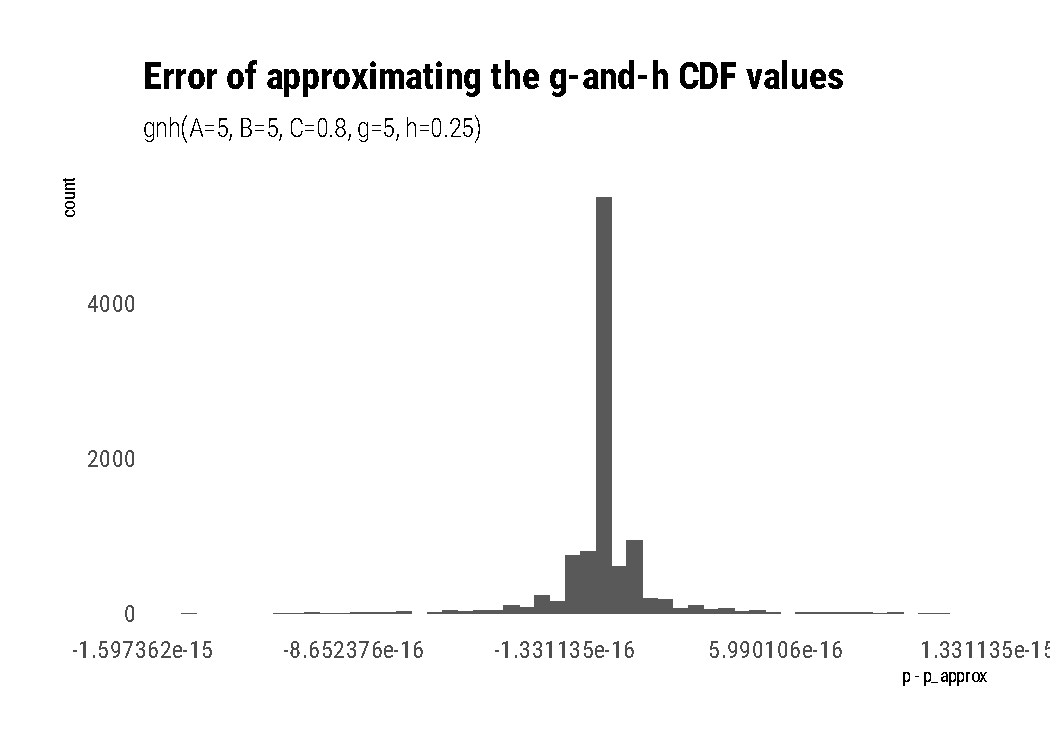
\includegraphics[width=0.5\linewidth]{ilbm_article_files/figure-latex/pgnk-error-1} 

}

\caption{Distribution of approximation error for g-and-h CDF values}\label{fig:pgnk-error}
\end{figure}

The absolute error of the approximation does not exceed \ensuremath{1.4432899\times 10^{-15}}. The desired precision can be set as the argument in \texttt{qpd::pgnh()}.

We take a sample of 100 simulated values from the g-and-h distribution with parameters A=5, B=5, C=0.8, g=5 and h=0.25. The distribution of simulated values is shown in Figure \ref{fig:gnh-data}.

\begin{figure}

{\centering 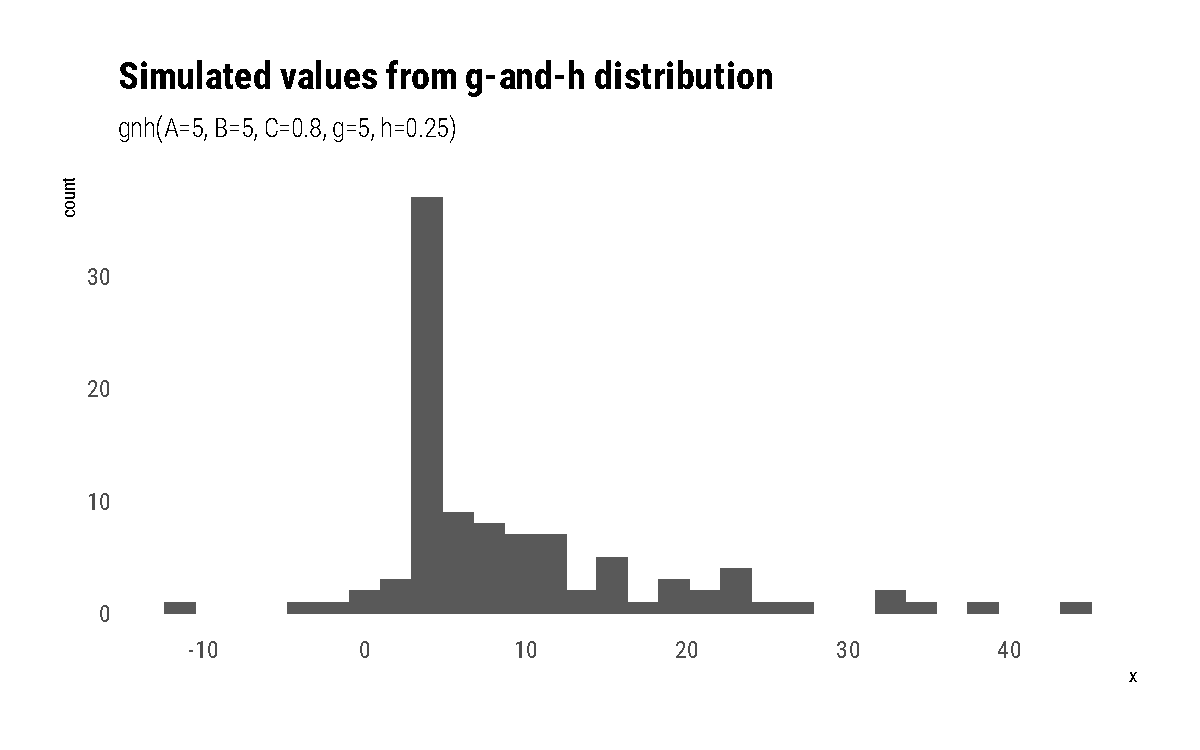
\includegraphics[width=0.5\linewidth]{ilbm_article_files/figure-latex/gnh-data-1} 

}

\caption{Simulated data from g-and-h distribution}\label{fig:gnh-data}
\end{figure}

We assumed that the parameters A and B of g-and-h distribution are known, and defined a normal prior for parameter \(g\) as \(Normal(3,1)\) and Rayleigh prior for parameter \(h\) as \(Rayleigh(0.3)\). We performed Bayesian inference using Robust Adaptive Metropolis MCMC algorithm by \citet{vihola2012RobustAdaptiveMetropolis} interfaced by the \texttt{fmcmc} package \citep{vegayon2019FmcmcFriendlyMCMC} in R. Table \ref{tab:gnh-fit-tbl} and Figure \ref{fig:gnh-combo-graph} summarize the posterior distribution of parameters \(g\) and \(h\).

\begin{table}[!h]

\caption{\label{tab:gnh-fit-tbl}Posterior summary of parameters in g-and-h distribution}
\centering
\begin{tabular}[t]{lrrrrr}
\toprule
variable & mean & median & q5 & q95 & rhat\\
\midrule
g & 4.9965104 & 5.011251 & 4.5878278 & 5.3899243 & 1.006485\\
h & 0.4248716 & 0.413202 & 0.2876798 & 0.5961615 & 1.002276\\
\bottomrule
\end{tabular}
\end{table}

\begin{figure}

{\centering 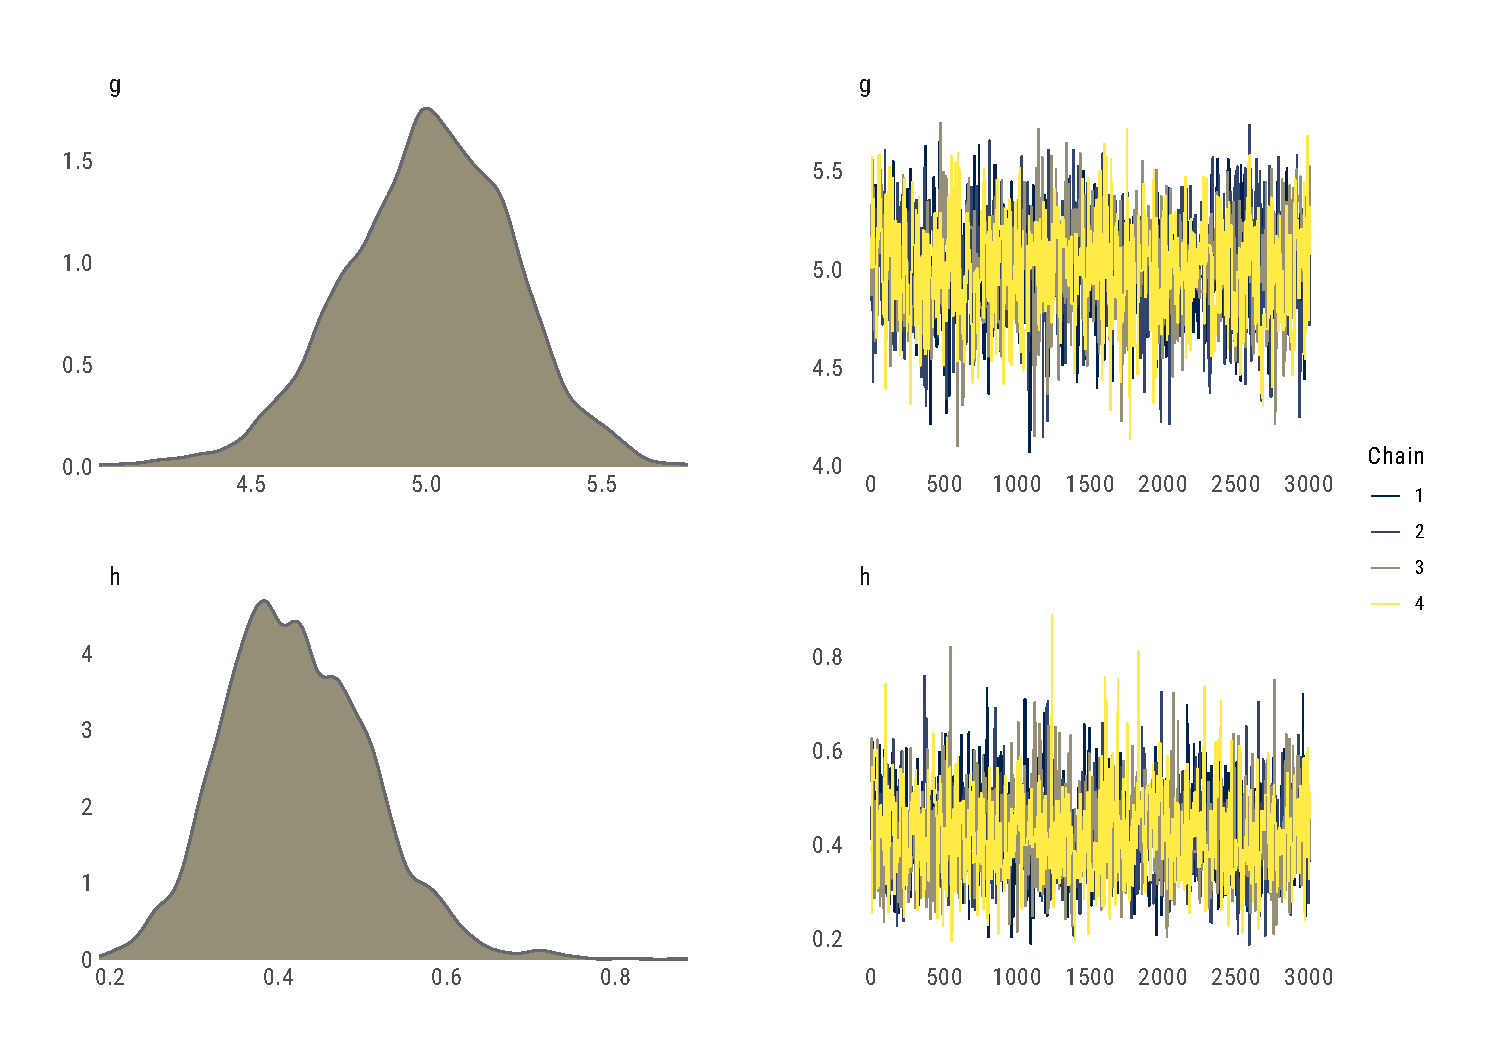
\includegraphics[width=0.8\linewidth]{ilbm_article_files/figure-latex/gnh-combo-graph-1} 

}

\caption{Posterior summary of parameters in g-and-h distribution}\label{fig:gnh-combo-graph}
\end{figure}

\hypertarget{validation-of-quantile-functions}{%
\section{Validation of quantile functions}\label{validation-of-quantile-functions}}

\begin{quotation}
This is a proofing window. When you approach the turnstile, you don't see yourself in the proofing window, do not enter the machine. \\
-- Ives in TENET by Christopher Nolan
\end{quotation}

Flexibility of quantile distributions can become their curse, as certain combination of parameters may produce an invalid quantile function. In order for the quantile function to be valid, it needs to be continuous and non-decreasing. Note that it is possible for a non-decreasing quantile function to produce a multi-modal density function (DQF) and still remain valid. The violation of the feasibility condition for the QF manifests itself in the negative values of the QDF, measuring the ``rate of change'' in the quantile function.

In some instances it is possible to avoid problematic cases by limiting the allowable range of values for the parameters. For example, \citet{prangle2017GkPackageGandk} and \citet{rayner2002NumericalMaximumLikelihood} discuss the range of valid parameter values for \emph{g-and-k} distribution. The parameter \(k\) shoud be larger than -0.5, but some values of \(k\), between -0.5 and 0 can also lead to a quantile function being invalid. The irregularities can be difficult to spot on the quantile function graph, but the effect on the derivative functions (QDF and DQF) can be quite dramatic.

\begin{figure}

{\centering 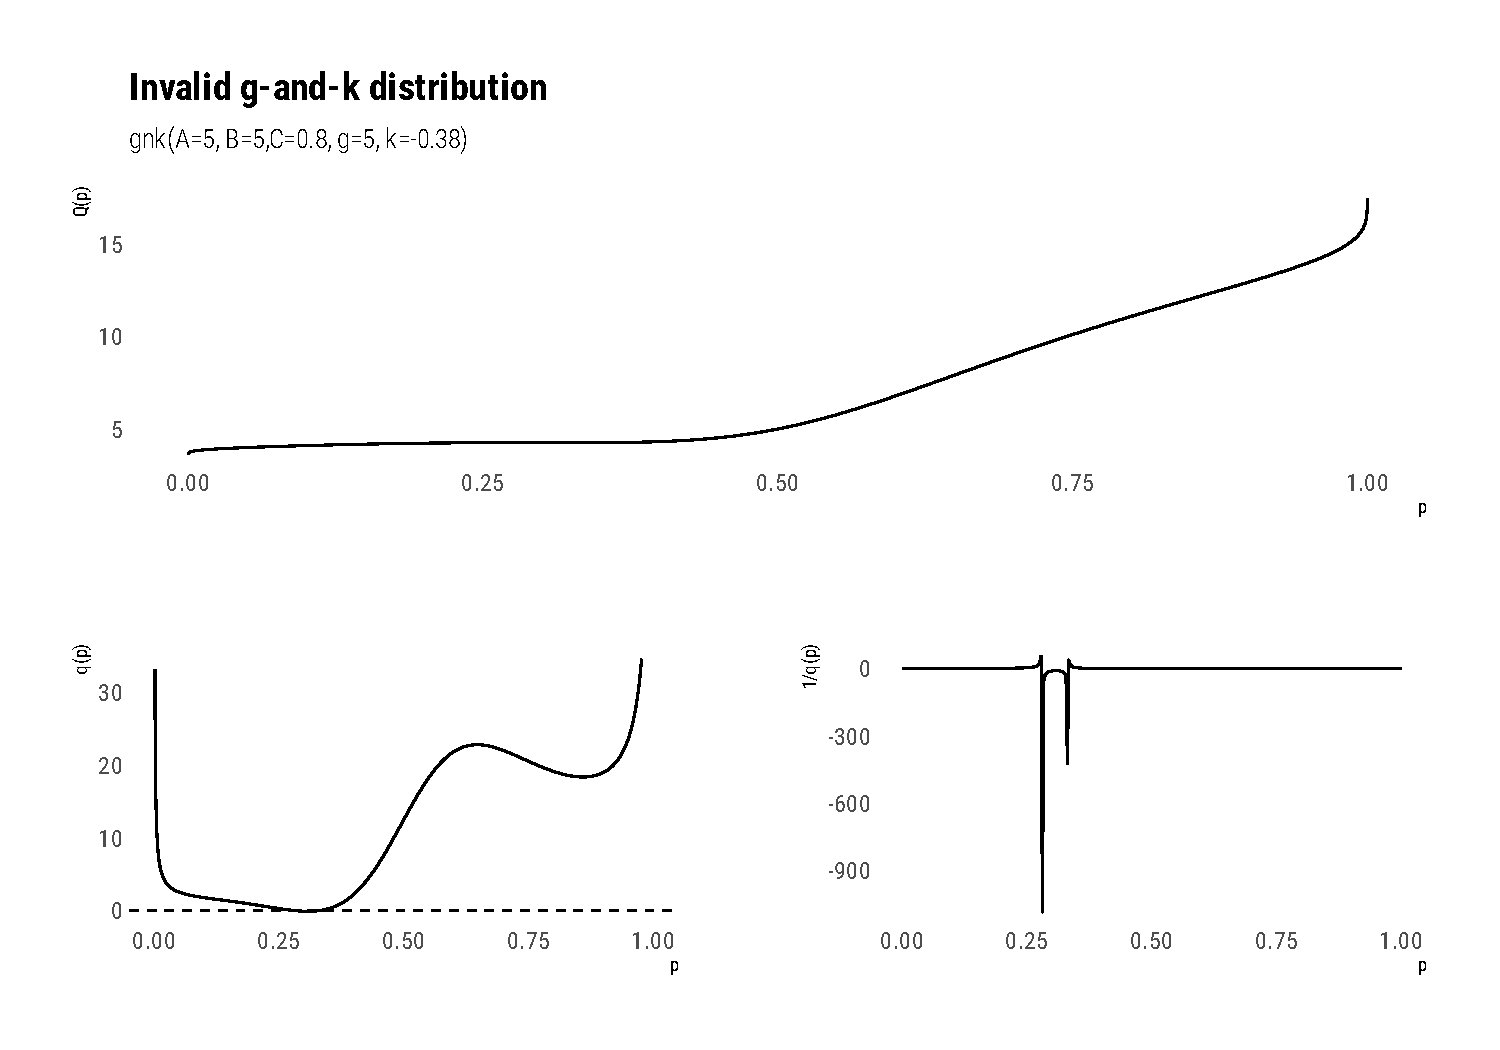
\includegraphics[width=0.8\linewidth]{ilbm_article_files/figure-latex/invalid-gnk-graph-1} 

}

\caption{Some combination of parameters of g-and-k distribution may lead to an invalid quantile function}\label{fig:invalid-gnk-graph}
\end{figure}

The invalid shape of the quantile function can cause the CDF approximation to fail both because the search (e.g.~using the Newton-Rhapson method) can get stuck in the local minima and because the QDF can produce an invalid gradient.

The validity of the quantile function can also be checked by computing the QDF values corresponding to the tight grid of probabilities spread across the {[}0,1{]} range. Should any one of the QDF values be negative we can reject the quantile function with there parameters as invalid. This requires that the probability grid is tight enough to eliminate the possibility of the QDF ``dipping'' below zero between the grid values. For a very tight probability grid, this method can be computationally expensive.

An alternative approach may include finding the global minimum of the QDF and checking if it is positive. However, given the complex shape of the QDF (Figure \ref{fig:invalid-gnk-graph}), this may prove to be computationally expensive as well.

A QDF can also be checked for roots. The values between the roots (or, if only one root is found, on one side of the root) are likely to be negative. Therefore if the roots are found this can indicate that the corresponding QF is invalid. The challenge with finding the QDF roots is that in most cases we can not use any of the bracketing methods, because the presence of roots is not known a-priori. The Newton-Rhapson method can also be problematic, due to difficulties of finding the ``good'' initial value. Also a gradient methods would require a derivative ``quantile convexity function'' (QCF) which may not be available, should the QDF be invalid. When validating the quantile function we are not interested in finding the roots per se, but rather in using them as an indication that a QDF may take negative values on the range {[}0,1{]} and thus, that the corresponding QF is invalid.

Finally, we can represent the QDF with a proxy function, the roots of which can be computed analytically. This method is referred to in the literature as the ``proxy root-finding'' and has been studied extensively \citep{boyd2013FindingZerosUnivariate}. Chebyshev polynomials are known for their ability to approximate functions of arbitrary complexity \citep{boyd2007NumericalExperimentsAccuracy}. In order to increase the precision of the approximation either higher degree polynomials should be used or the function range should be paritioned, keeping the degree of the polynomials applied on the subdivisions low. \citet{boyd2006ComputingRealRoots} discusses two methods correponding to these strategies. The first of them referred to as the ``tredecic method'', envisages that regardless of number of partitions the polynomial of fixed degree (M=13) is used. The other method called ``megacubes'' refers to applying a low-degree polynomial on a very large number of partitions (enumerated in thousands). The main computational load of the Chebyshev polynomial method is computing the eigenvalues of the Chebyshev-Frobenius companion matrix \citep{boyd2013FindingZerosUnivariate}. The logic of the ``megacubes'' method (and any method relying on a large number of paritions) is that it might be computationally cheaper to find eigenvalues of many small matrices, than computing eigenvalues of a large matrix. The \texttt{qpd} package \citep{perepolkin2019QpdToolsQuantileparameterized} implements several functions for computing the coefficients, finding roots and evaluating the Chebyshev polynomial of arbitrary degree on any interval of a function. For QPD the full range of the function is \((0,1)\), but \texttt{qpd::is\_qpd\_valid()} can check a qpd function passed by the user on arbitrary number of subdivisions (using either uniform or an S-shaped subdivision scheme) automating the process of subdividing the range of a function and fitting the Chebyshev polynomial of a user-defined degree to every partition.

When using high degree polynomials on complex QPDs false-positives are not uncommon. \citet{boyd2006ComputingRealRoots} suggests using the roots identified by the proxy-rootfinding method as starting values for the Newton-Rhapson algorithm to refine (or refute the presence of) the roots. This adds to computational complexity and requires the presence of a valid QCF. The method adopted by the \texttt{qpd} package is based on the idea of using the proxy roots as subdivisions of a QDF (0,1) range and checking one value from every segment of the function range formed by the proxy roots (e.g.~if only one proxy root is found, two values, - one on each side of the root).

\begin{figure}

{\centering 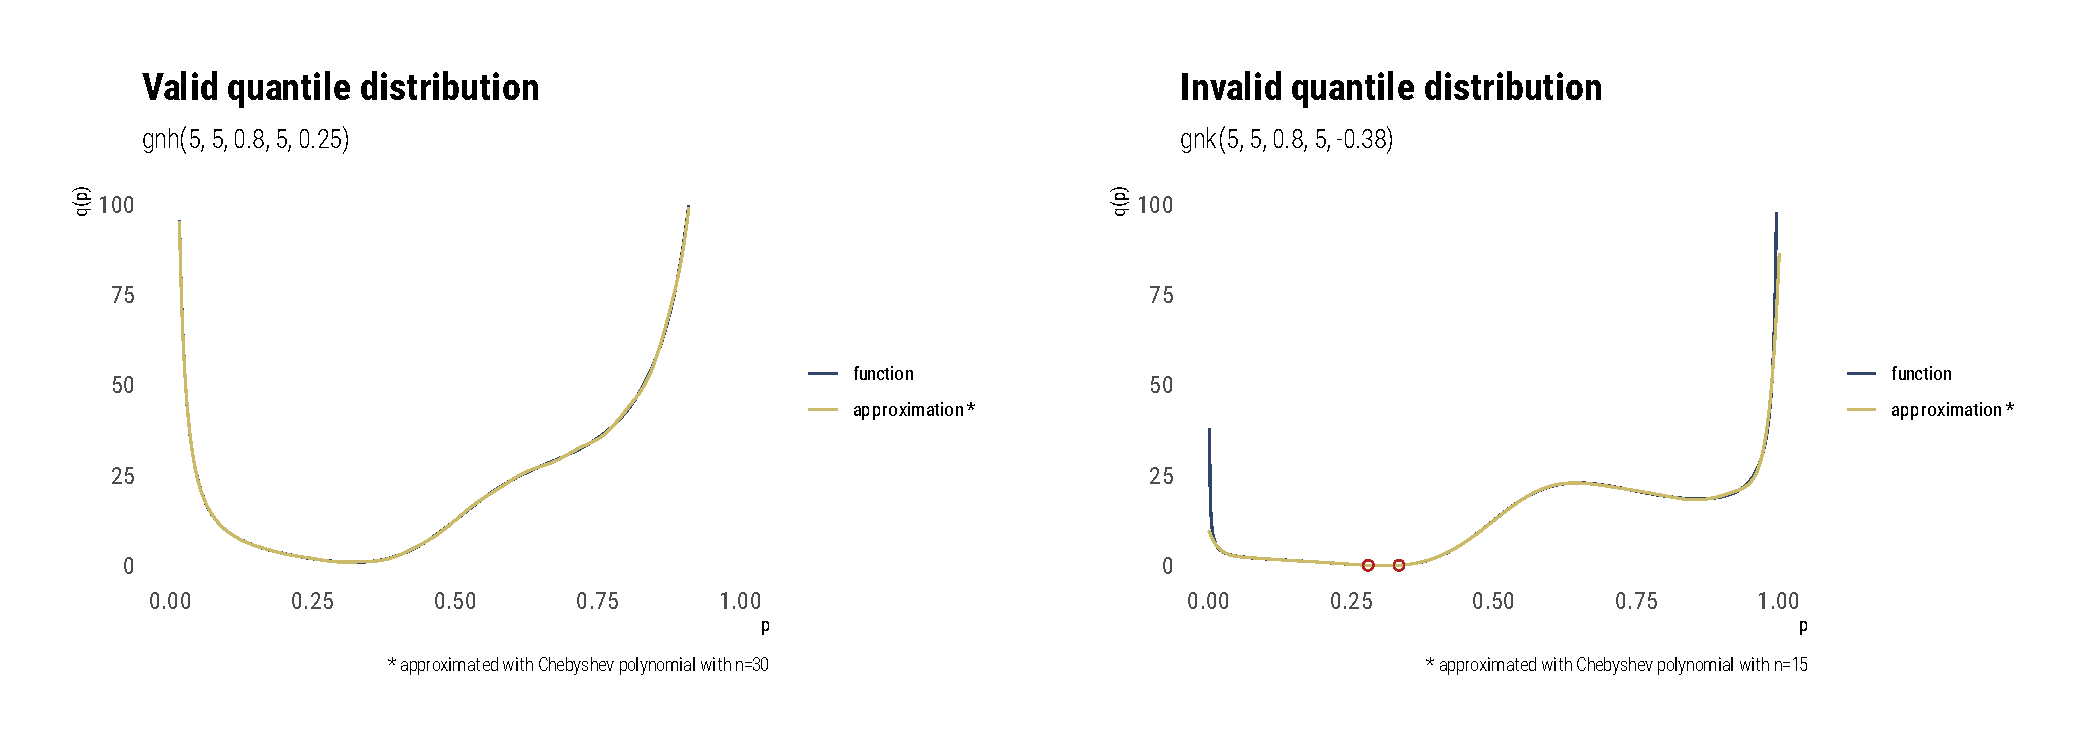
\includegraphics{ilbm_article_files/figure-latex/chebyshev-roots-funs-1} 

}

\caption{Chebyshev polynomial approximation for validating two quantile distributions}\label{fig:chebyshev-roots-funs}
\end{figure}

Figure \ref{fig:chebyshev-roots-funs} shows a valid and an invalid QDF, with the presence of two roots on the latter. The complexity of the polynomial varies and can be optimized using the OLS. Moreover, if the QDF range is partitioned into the smaller segments, then much lower degree polynomial can be applied on each interval.

\begin{quote}
\textbf{DP Comments:}

\begin{itemize}
\item
  For the Specialized distributions I have the flood flow dataset, which has its own distribution - Wakeby, which was developed for modeling of floods or thunderstorms. Wakeby has crazy parametrization (many impossible combinations of parameters) so it would be cool to discuss how it can be done in Stan.
\item
  Especially when we talk about indirect priors, they make sense almost solely in the context of QPDs, ie when we have expert-elicited assessment of parameters. For Wakeby distribution there are some parameters from the published papers and some can just be given by opinion. I am hesitant to introduce any of the QPDs in this paper. Lets keep that Pandora box locked until the second paper.
\item
  I can easily include small snippets of code if that is considered educational. Just need to find a way of not being overwhelming. All models are in the \texttt{stan/} folder in the repo.
\end{itemize}
\end{quote}

\hypertarget{discussion}{%
\section{Discussion}\label{discussion}}

\begin{quotation} 
You are inverted, the world is not. \\ 
-- Wheeler in TENET by Christopher Nolan
\end{quotation}

Here some of the ideas for which I can write a paragraph or two of discussion.

\hypertarget{moebius-loop-of-the-probability-functions}{%
\subsection{Moebius loop of the probability functions}\label{moebius-loop-of-the-probability-functions}}

maybe this can be moved upfront

\hypertarget{practical-tips-for-implementing-quantile-distributions-in-stan-and-in-r.}{%
\subsection{Practical tips for implementing quantile distributions in Stan and in R.}\label{practical-tips-for-implementing-quantile-distributions-in-stan-and-in-r.}}

\hypertarget{finding-good-initial-values}{%
\subsection{Finding good ``initial values''}\label{finding-good-initial-values}}

Challenges with grid-matching in Stan (divergences)

\hypertarget{root-finding-algorithms-in-stan-and-r}{%
\subsection{Root-finding algorithms in Stan and R}\label{root-finding-algorithms-in-stan-and-r}}

Numerical inversion of QF is ``the CDF pincer movement''.
\texttt{nlm()}? numerical derivatives? For Stan I just want to rant that there's still no built-in 1D rootfinder.

\hypertarget{performance-tradeoffs-with-chebyshev-polynomials}{%
\subsection{Performance tradeoffs with Chebyshev polynomials}\label{performance-tradeoffs-with-chebyshev-polynomials}}

This is worth a separate paper and a lot has been written, so just citing the literature. Reality is that it is expensive and loses to the tight grid for QDFs of moderate complexity. Needs implementation in C++.

\hypertarget{expert-specified-indirect-priors}{%
\subsection{Expert-specified indirect priors}\label{expert-specified-indirect-priors}}

This will hint towards the quantile-parametrized quantile distribution, foreshadowing the next paper.

  \bibliography{ilbm-article.bib}

\end{document}
